\chapter{Diseño del brazo robótico: Punto de inicio} \label{chap:Punto_partida}
\chapterimage{figuras/ImagenesPortada/PortadaDisenoGeneral.jpg}

En este capítulo se continuará perfilando los aspectos de diseño generales del prototipo. Una vez repasado el estado del arte en el capítulo \ref{chap:estadoarte} ya se tiene una idea de las soluciones disponibles y sus deficiencias y fortalezas. Este capítulo vuelve sobre los objetivos presentados en el capítulo \ref{chap:Introduccion} para ofrecer un marco más completo sobre el que se apoye todo el desarrollo del proyecto así como posteriores capítulos.
\\

Es importante recordar que el prototipo debe estar en constante interacción con usuarios no especializados; es por ello que se han preestablecido unas características básicas que suponen un afianzamiento de la seguridad hacia los usuarios inherentes al diseño.

\begin{itemize}
    \item Se impone el uso de motores con bajo par de trabajo. De esta manera se vuelve físicamente imposible que los mismos puedan suponer un riesgo para los usuarios ya que la fuerza que son capaces de realizar no es suficiente para suponer un peligro para los mismos.
    \item El uso de motores de bajo par implica una compensación del peso del propio brazo de forma que los motores deban cargar con el meonr peso posible. Eso se consigue a través de mecanismos de cuatro barras acoplados, de igual forma que se hace en diferentes lupas y lámparas comerciales como se puede ver en la figura \ref{fig:PuntoPartida:CuatroBarras}. Como demuestra \cite{Rahman_asimple} compensar este tipo de estructuras mediante el uso de muelles es bastante sencillo sea cual sea el número de articulaciones que acopladas.
    \begin{figure}
    	\centering
    	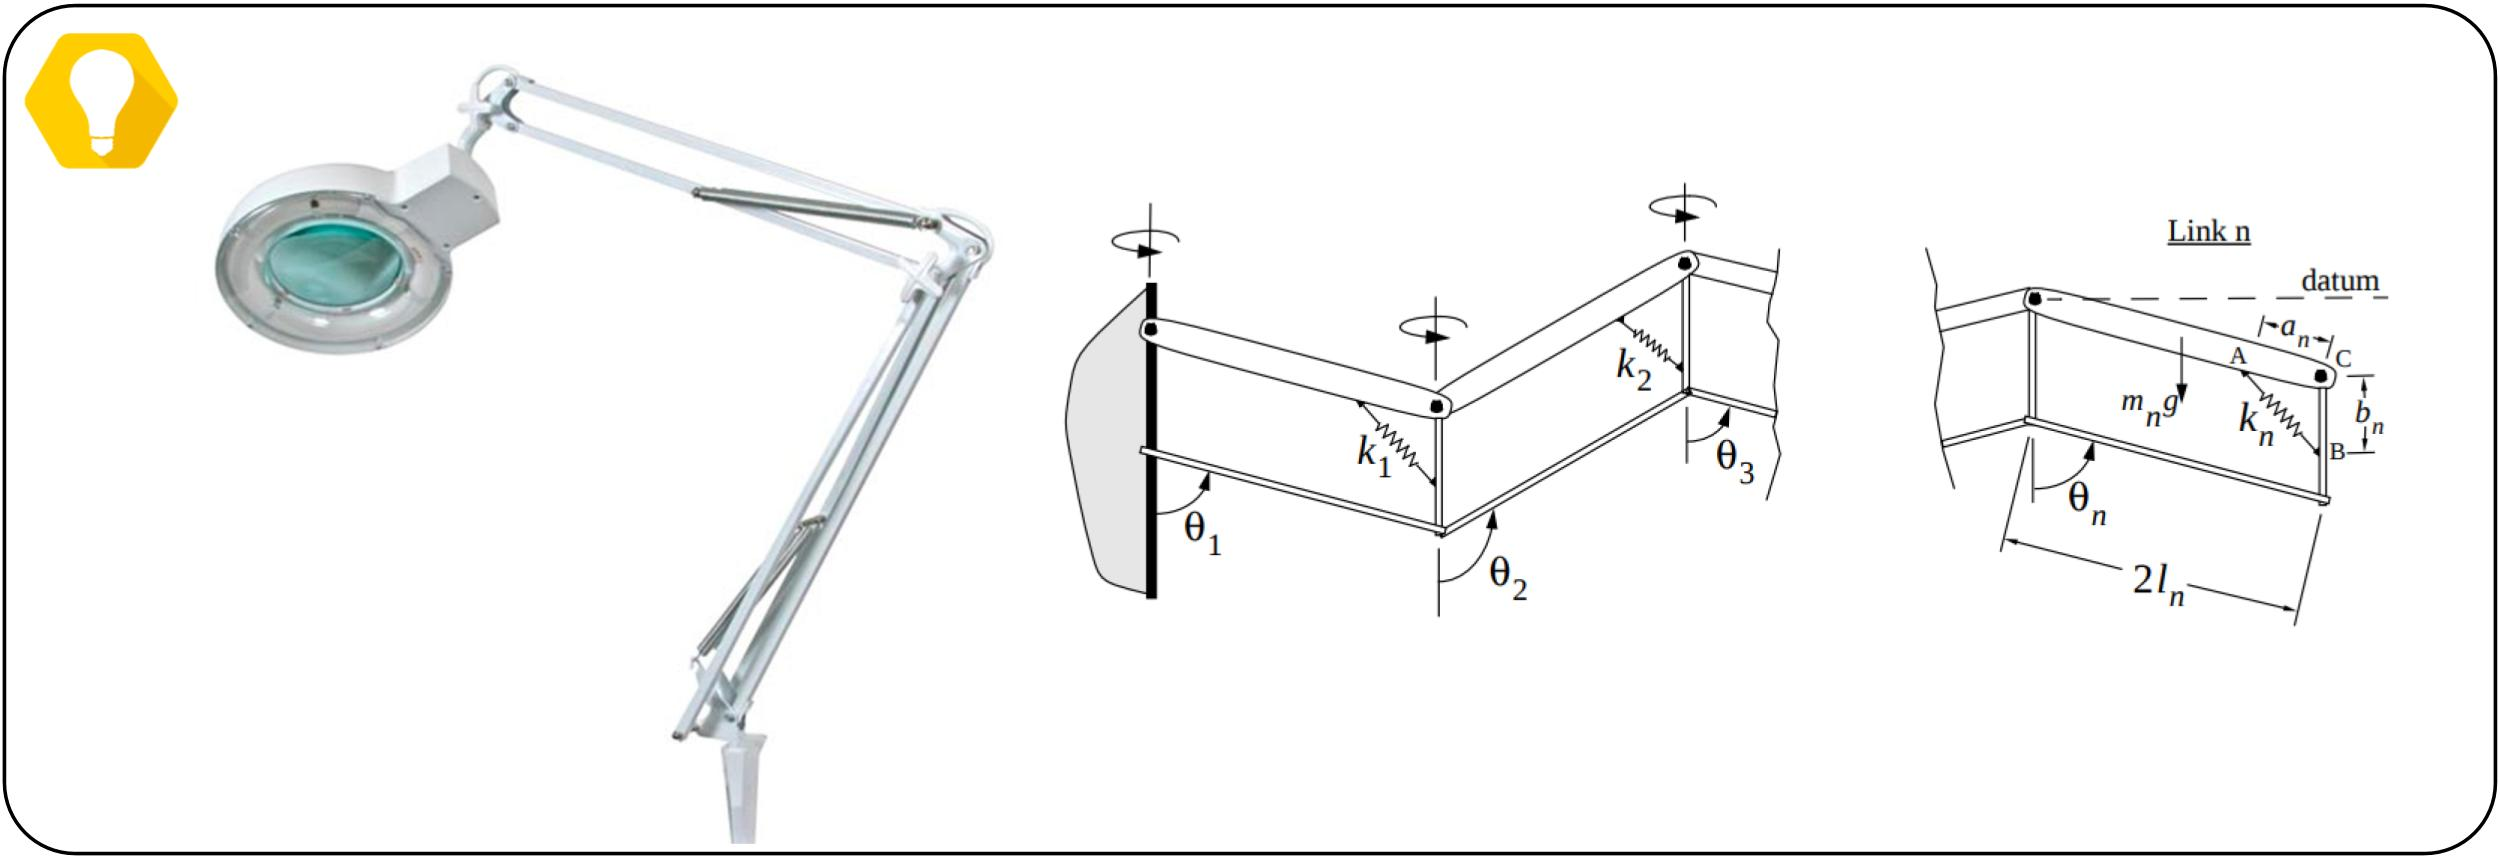
\includegraphics[width=1\textwidth]{figuras/Imagenes_PuntoPartida/CuatroBarras.jpg}
    	\caption{Ejemplos de como se acoplan y compensan estructuras basadas en mecanismos de cuatro barras}
    	\label{fig:PuntoPartida:CuatroBarras}
    	\immagesource{A la izquierda imagen de internet. A la derecha es una captura de \cite{Rahman_asimple}}
    \end{figure}
    \item Además la elección de dichos motores implica una amplificación mecánica a lo largo de la transmisión del movimiento en el diseño del prototipo. Los motores estarán ubicados en la base y el par de los mismos será transmitido a las articulaciones. Se ha optado por una transmisión mediante hilos que, como dice \cite{LeonardoCodice} será siempre más silenciosa y suave, permitirá hacer la transmisión solo en un sentido, es decir, para subir el extremo del brazo (figura \ref{fig:PuntoPartida:leonardo}). El sentido de bajada se hará soltando dicho hilo dejando que la gravedad y el peso del brazo lo hagan descender. De esta manera en caso de que se encuentre un usuario en la trayectoria del brazo éste no podrá ejercer una fuerza activa contra el mismo. El paciente sentirá como mucho como el peso del brazo, compensado en su mayoría mediante los muelles, se apoya sobre si mismo.
    \begin{figure}[H]
    \begin{adjustwidth}{-1.9cm}{-1.5cm}
           \centering
           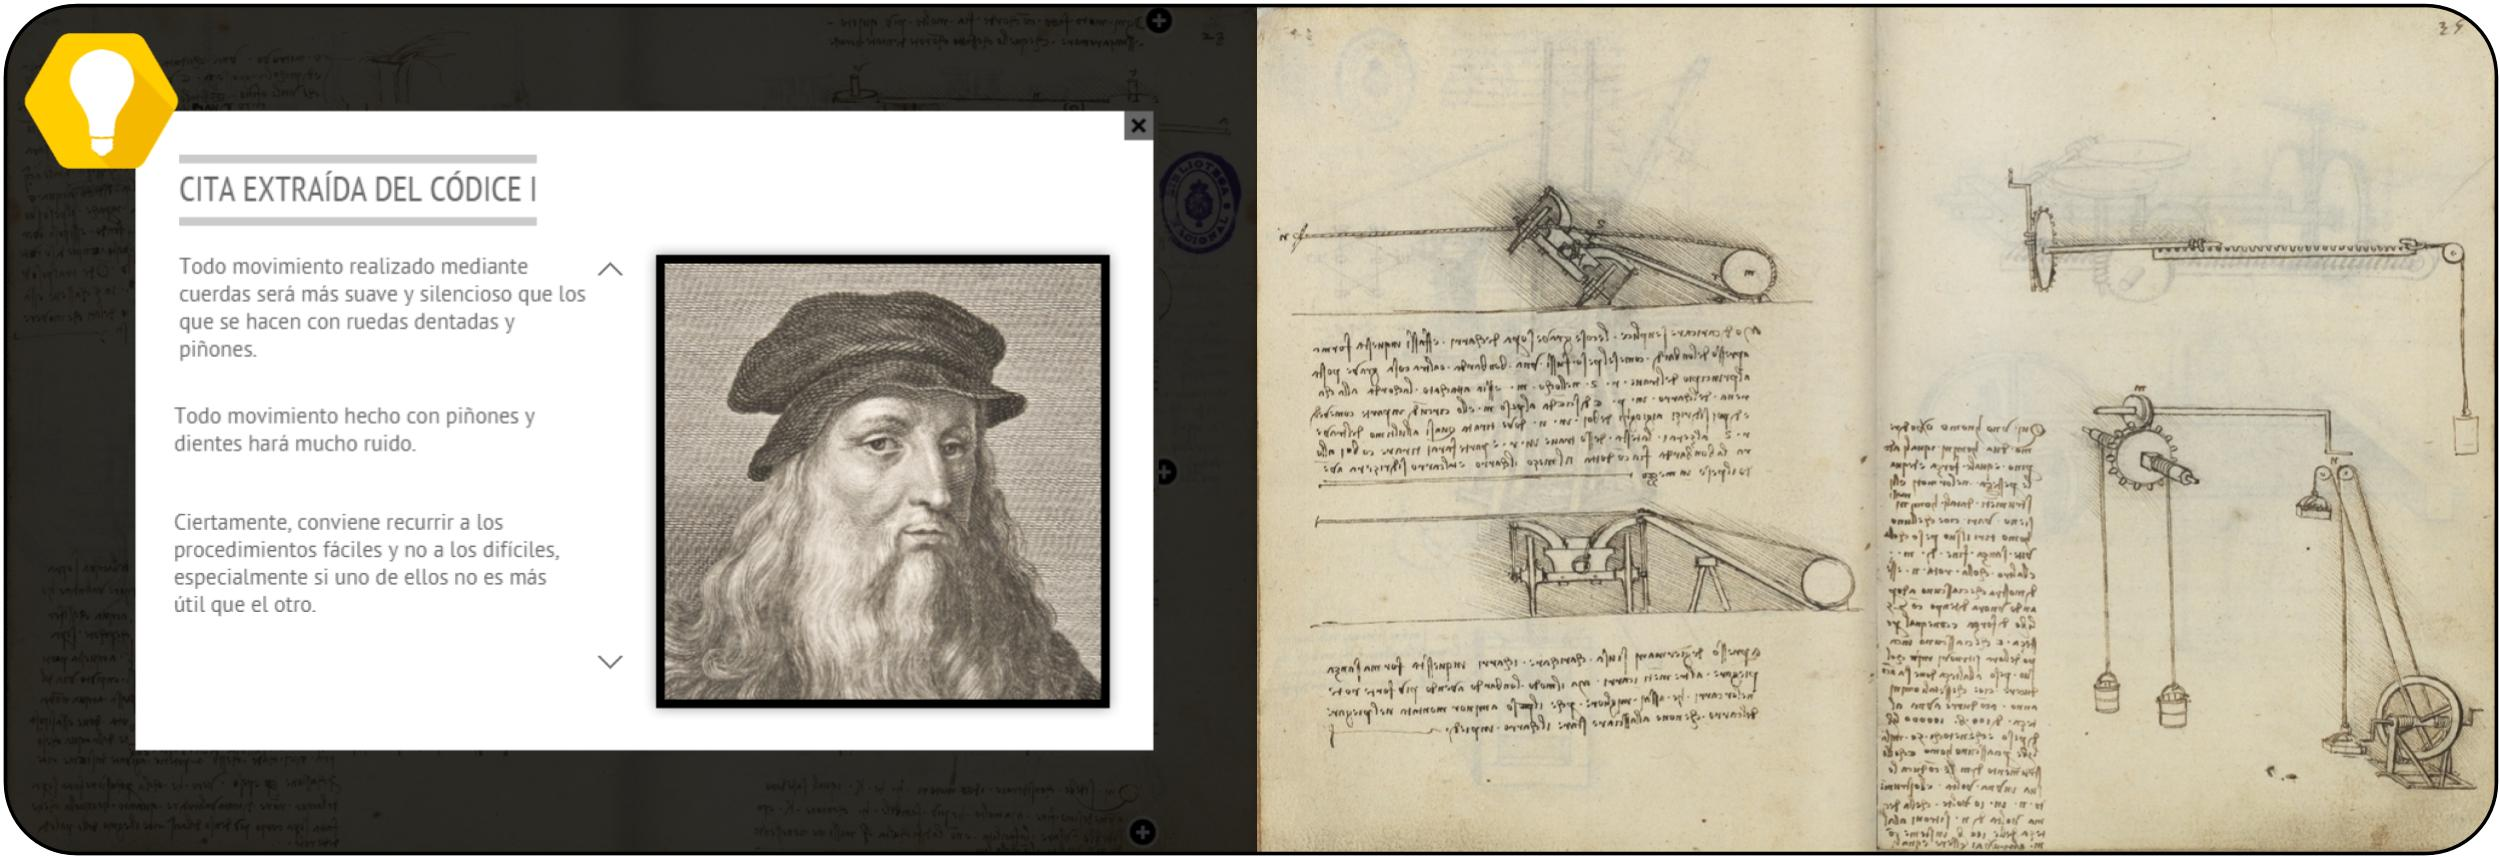
\includegraphics[width=1.1\textwidth]{figuras/Imagenes_PuntoPartida/Leonardo.jpg}
           \caption{Captura del documento original digitalizado de \cite{LeonardoCodice}}
           \label{fig:PuntoPartida:leonardo}
           \immagesource{Captura de \cite{LeonardoCodice}}
       \end{adjustwidth}
    \end{figure}
    \item El uso de hilos para la transmisión permitirá además una reversibilidad en el control efectuado. Otra posible alternativa es la transmisión del movimiento por rozamiento, de forma que el usuario no sufrirá daño alguno en cuanto la fuerza que haga el mismo sobre el robot supere el rozamiento de dicha transmisión.
\end{itemize}

Como pruebas de concepto, puesto que el diseño de una versión completa lleva una cantidad de tiempo y de trabajo nada despreciables se ha hecho uso de diferentes maquetas diseñadas específicamente para probar algunas estructuras mecánicas que formarán parte de la estructura del robot. Algunos métodos sobre los que se puede apoyar la construcción de maquetas, siempre a escala, son la impresión 3D (maquetas en plástico) o el corte láser (maquetas en madera DM). De esta forma se realizan de forma rápida y barata pruebas de concepto para descartar o incluir diferentes ideas en el diseño final. Algunas maquetas realizadas para pruebas de concepto de la estructura mecánica se pueden ver en la figura \ref{fig:PuntoPartida:maquetas}.

\begin{figure}[H]
    \centering
    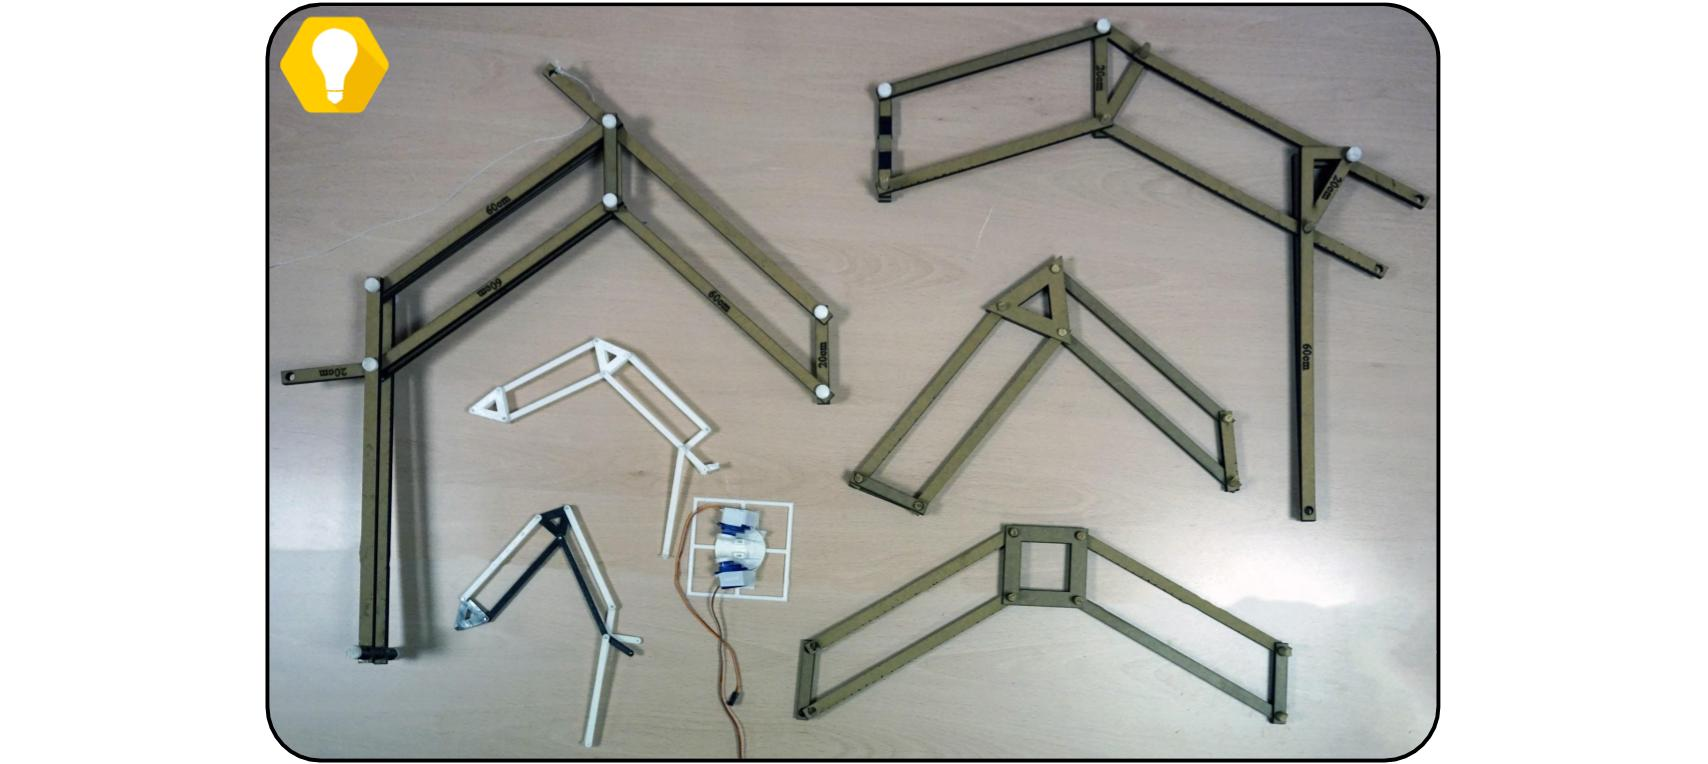
\includegraphics[width=1\textwidth]{figuras/Imagenes_PuntoPartida/maquetas.jpg}
    \caption{Maquetas en plástico y madera DM}
    \label{fig:PuntoPartida:maquetas}
    \immagesource{Autor}
\end{figure}

Aun haciendo uso de maquetas, y como en cualquier proyecto de prototipo, ha sido necesario seguir una metodología iterativa. Para los diferentes aspectos del proyecto se van probando y corrigiendo diferentes aspectos de la mecánica e integración de los componentes de forma que se va refinando y completando un modelo definitivo. Como ejemplo se puede ver en la figura \ref{fig:PuntoPartida:rovbolution} como ha ido evolucionando el desarrollo mecánico que se verá a continuación.
\\

\begin{figure}[H]
    \vspace{-1cm}
    \begin{adjustwidth}{-1.9cm}{-1.5cm}
       \centering
       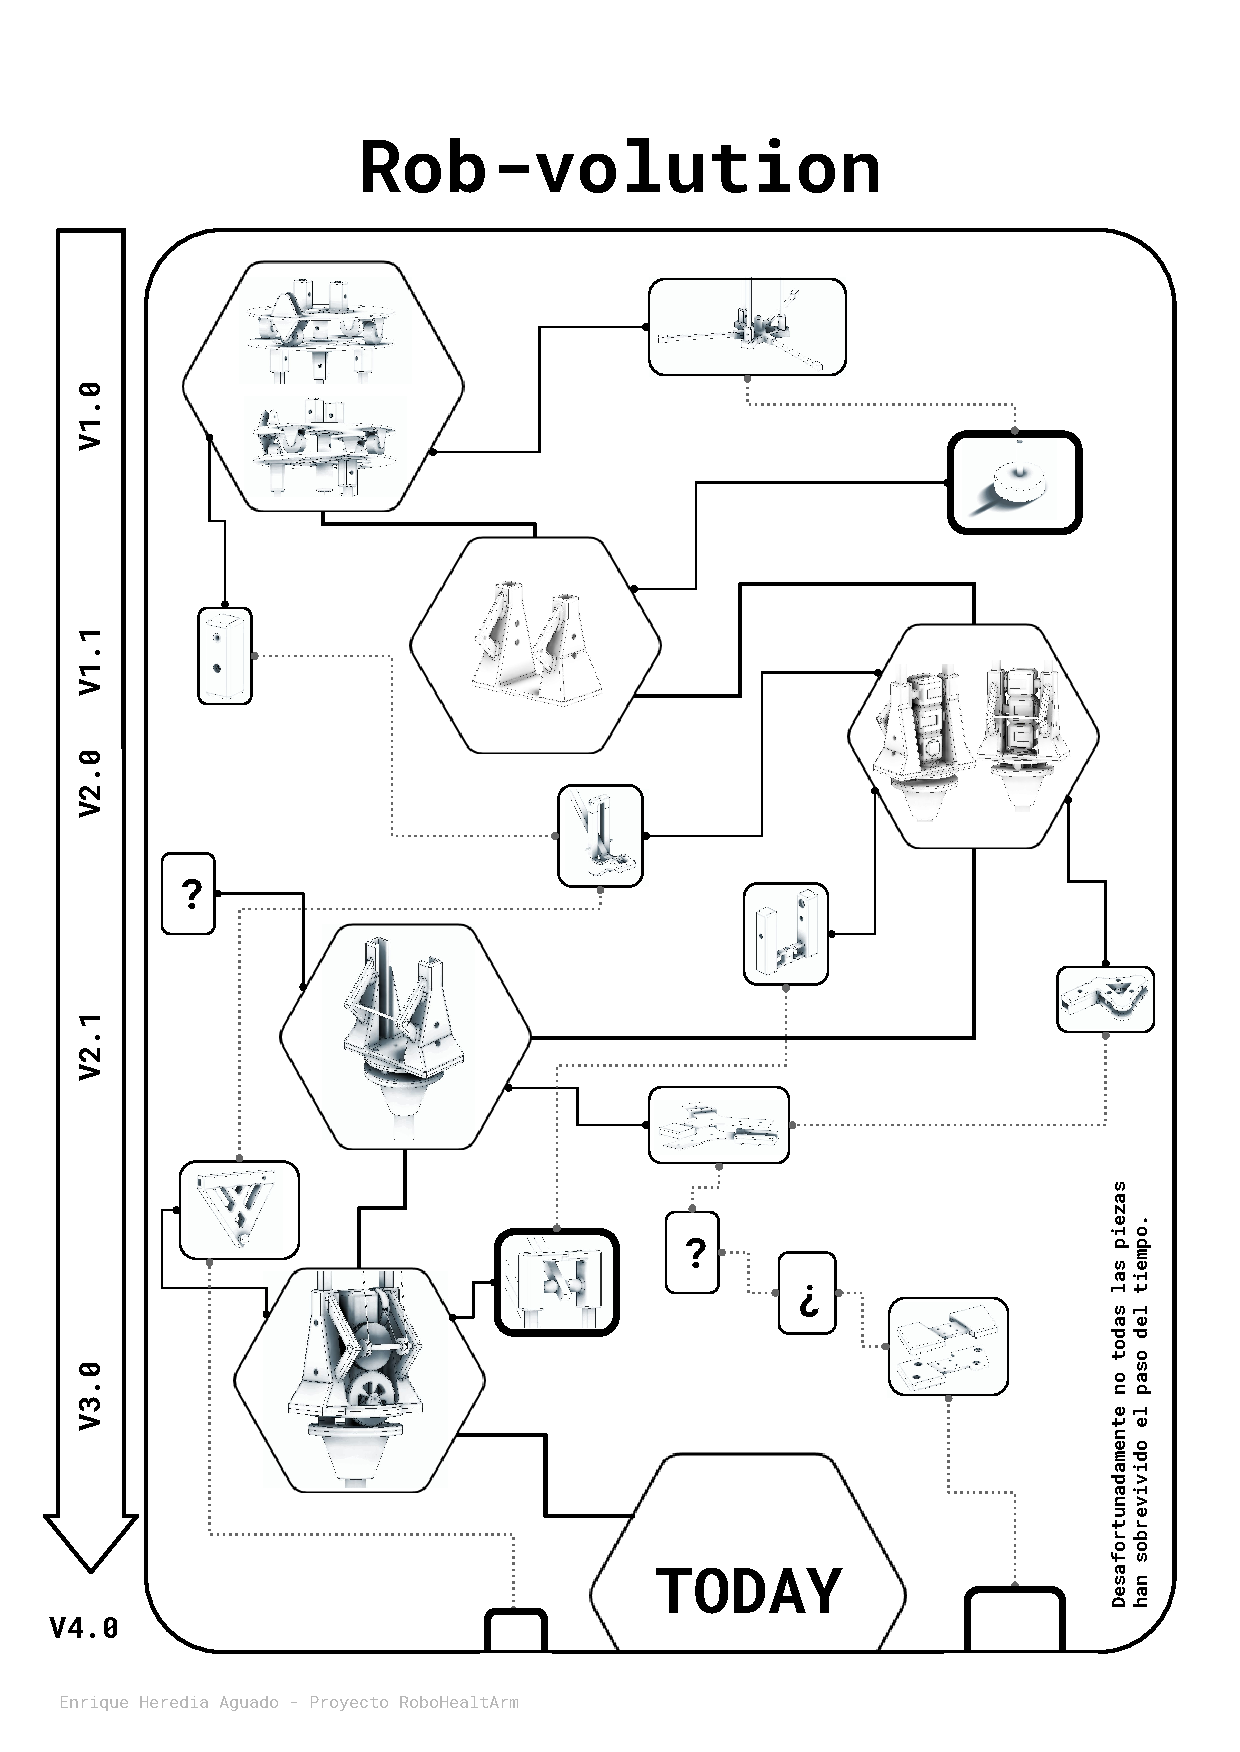
\includegraphics[width=1.1\textwidth]{figuras/Imagenes_PuntoPartida/Rob-volution.pdf}
       \caption{Esquema de la evolución de diferentes versiones del diseño mecánico}
       \label{fig:PuntoPartida:rovbolution}
       \immagesource{Autor}
   \end{adjustwidth}
\end{figure}

Como es de esperar, un proceso iterativo de este tipo acaba por generar un \textit{cementerio} de piezas desechadas y actualizadas a modelos más completos y mejorados.

\begin{figure}
   	\centering
   	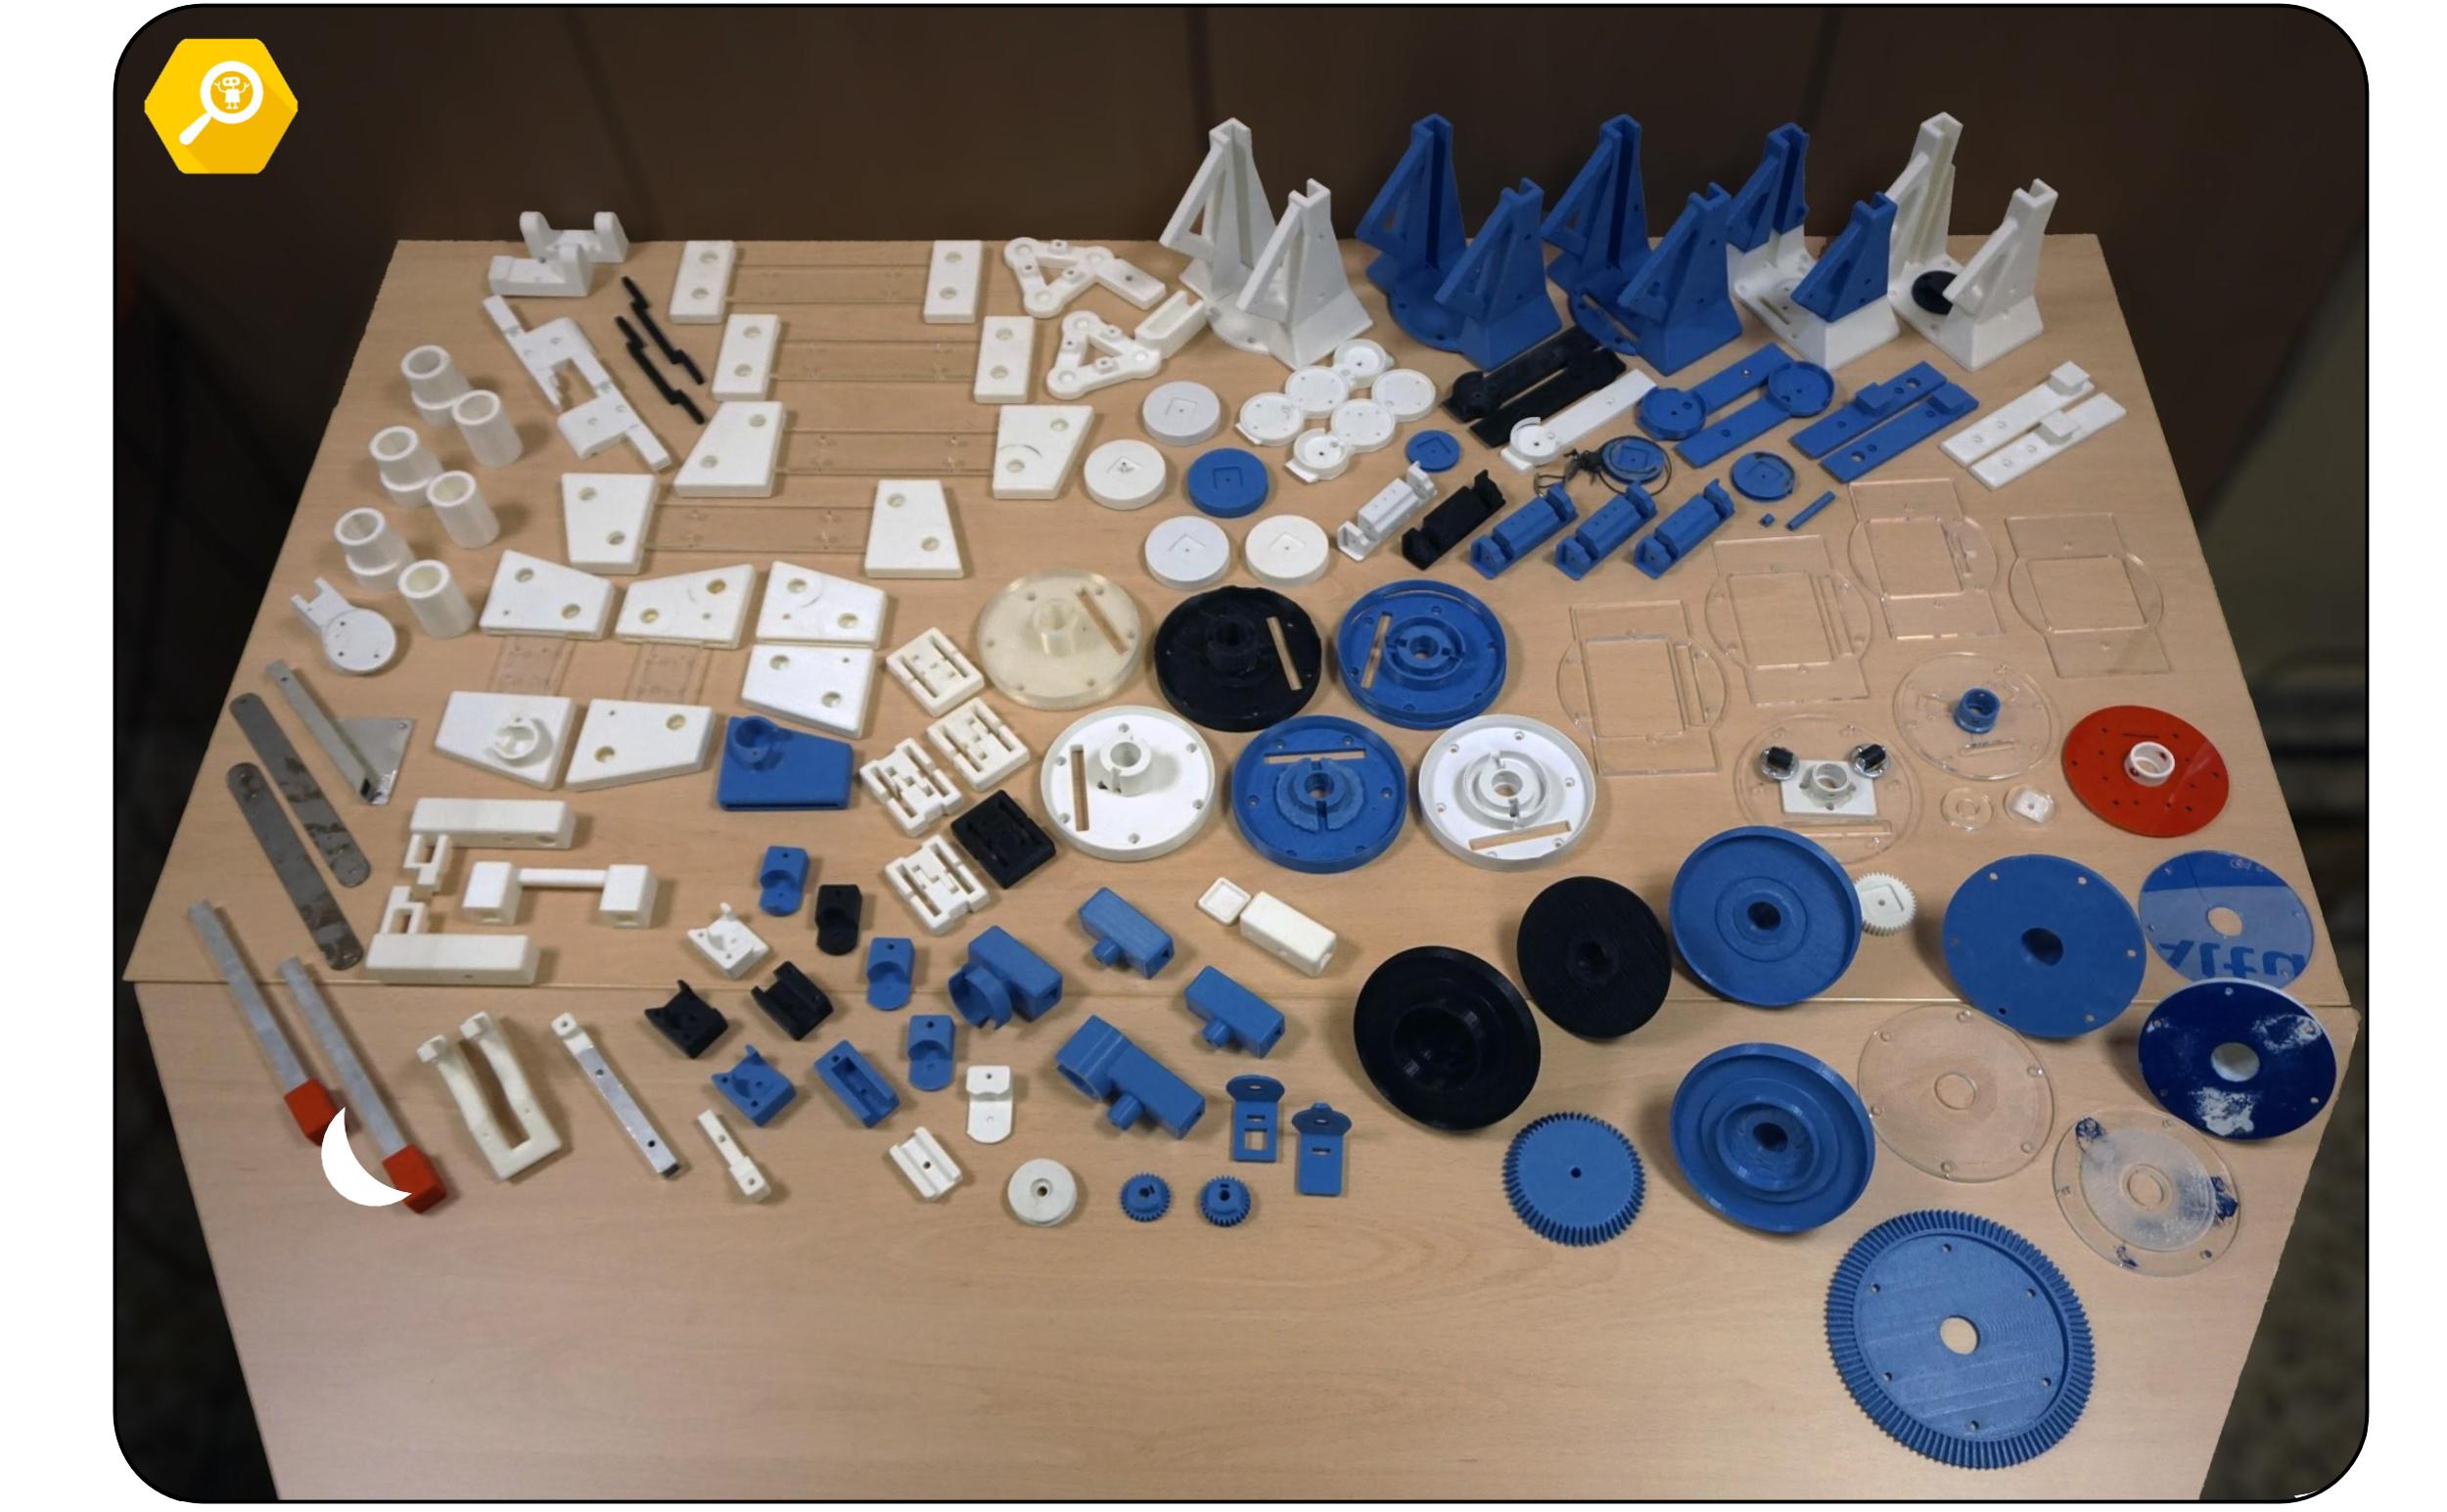
\includegraphics[width=1.1\textwidth]{figuras/Imagenes_PuntoPartida/cementerio.jpg}
   	\caption{Piezas previas al diseño definitivo}
   	\label{fig:PuntoPartida:cementerio}
   	\immagesource{Autor}
\end{figure}
%\includegraphics{myfig.pdf}
%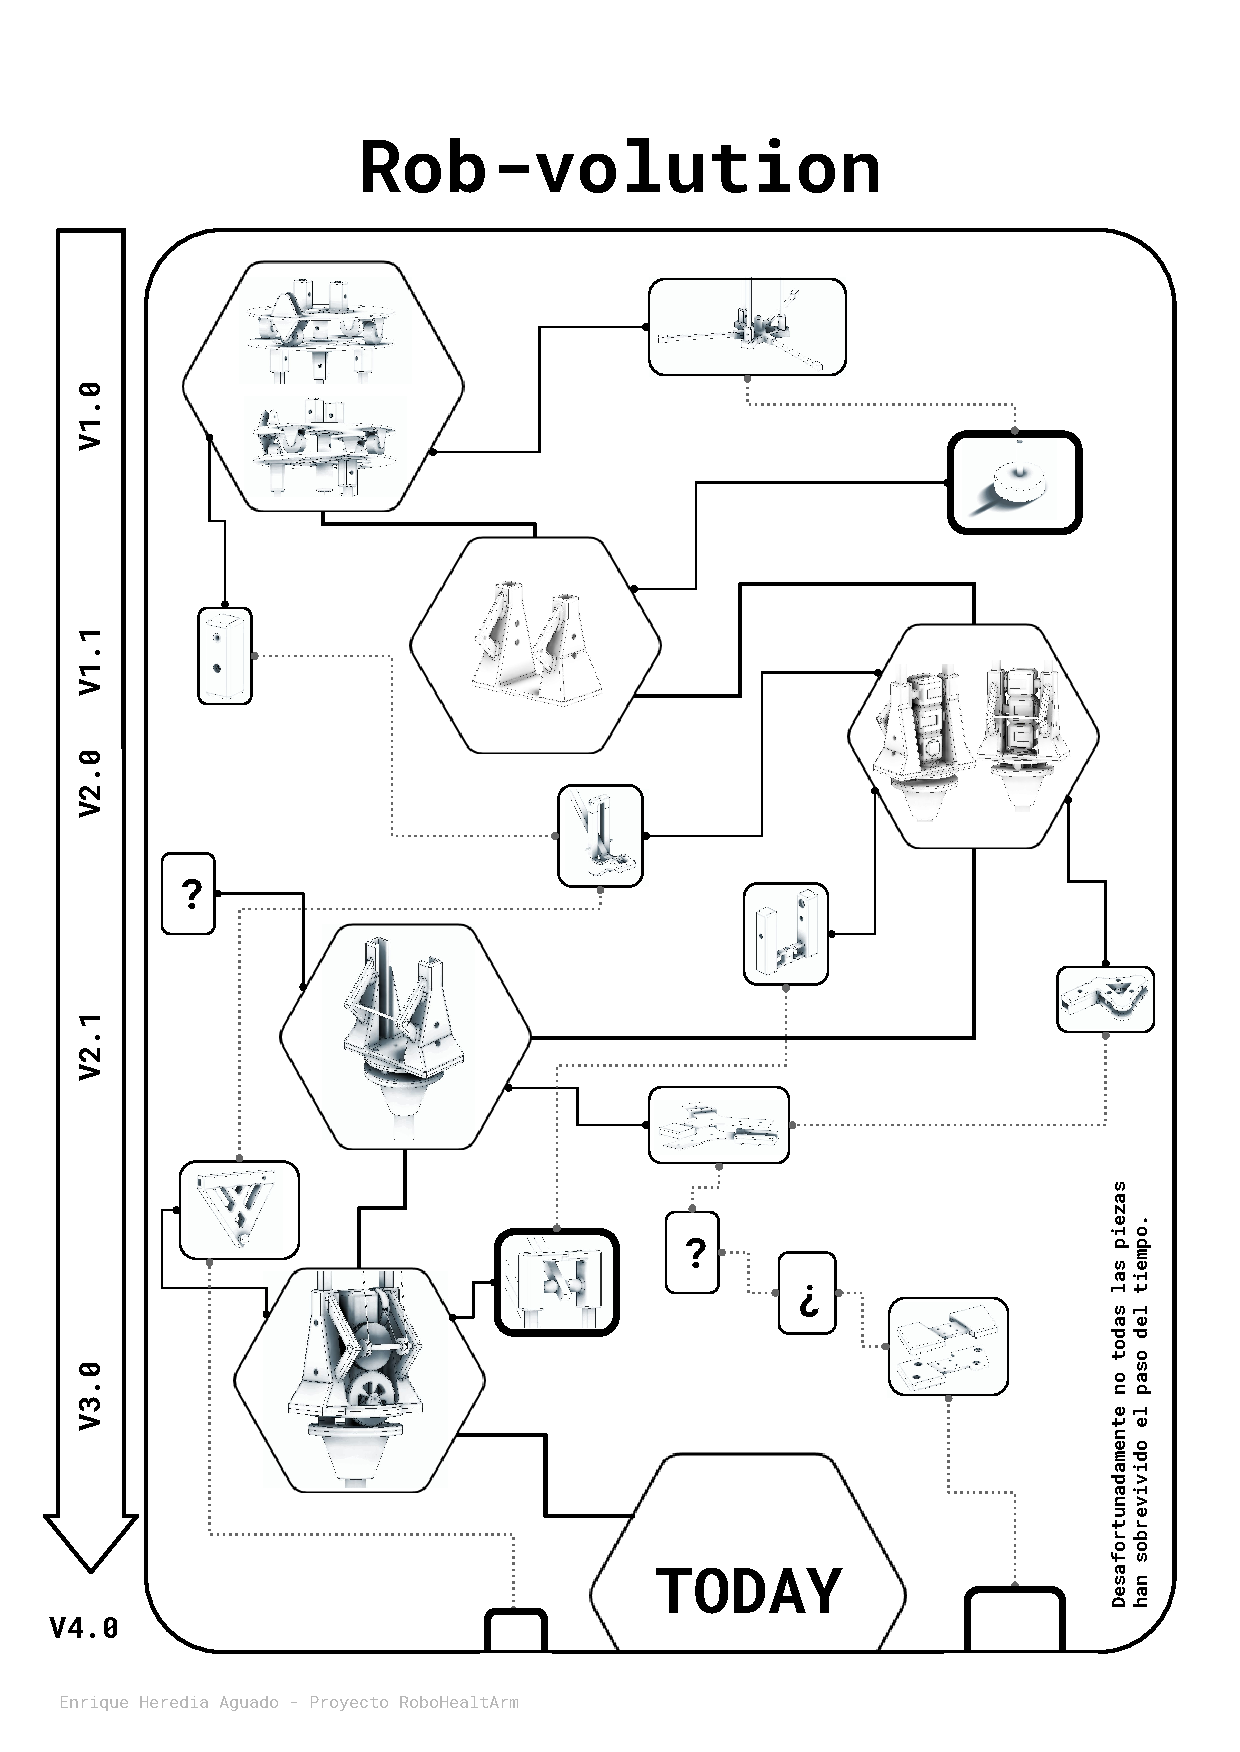
\includepdf[pages={1}]{figuras/Imagenes_PuntoPartida/Rob-volution.pdf}
